\documentclass[11pt,a4paper]{article}
\usepackage{polski}
\usepackage[utf8]{inputenc}
\usepackage{listings}
\usepackage{graphicx}
\usepackage{color}
\renewcommand{\floatpagefraction}{0.1}
\title{Dźwięk i muzyka w systemach komputerowych - laboratorium 03}
\author{Marcin Fabrykoski}
\date{}
\begin{document}
\maketitle
\newpage
\begin{enumerate}
\item Naszym zadaniem jest przeprowadzić analizę widmową wybranych instrumentów muzycznych używając przygotowanych sampli.\\
Poniżej przedstawiony jest program realizujący to zadanie dla kamertonu:
\lstinputlisting[language=Octave,basicstyle=\footnotesize,caption="Zadanie 1"]{zad1.m}
Wyniki widać odpowiednio na rysunkach:
\begin{enumerate}
\item akordeon rys.\ref{fig:akordeon}
\item flet rys.\ref{fig:flet}
\item fletnia rys.\ref{fig:fletnia}
\item kamerton rys.\ref{fig:kamerton}
\end{enumerate}
\begin{figure}
\hspace{-10em}
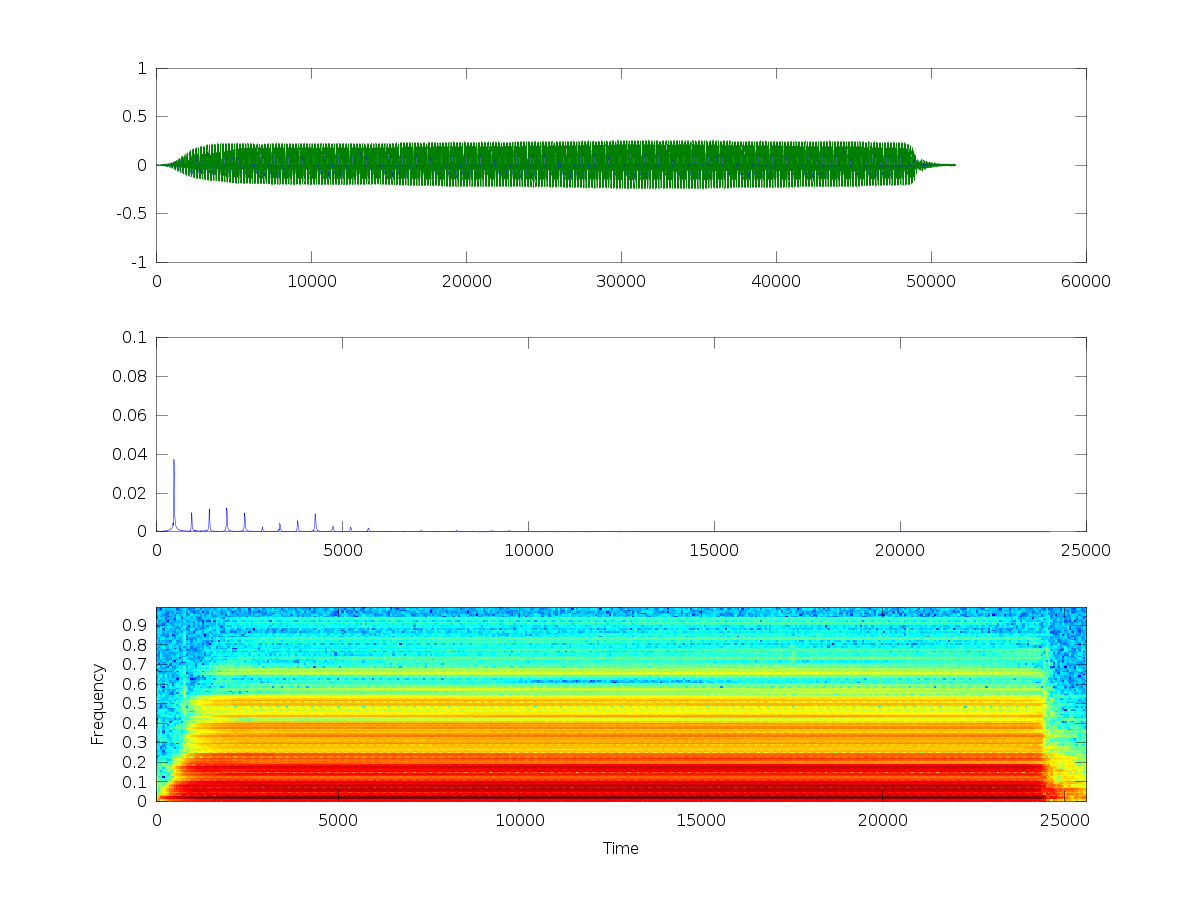
\includegraphics[scale=0.5]{proba1_akordeon.png}
\caption{Akordeon}
\label{fig:akordeon}
\end{figure}
\begin{figure}
\hspace{-10em}
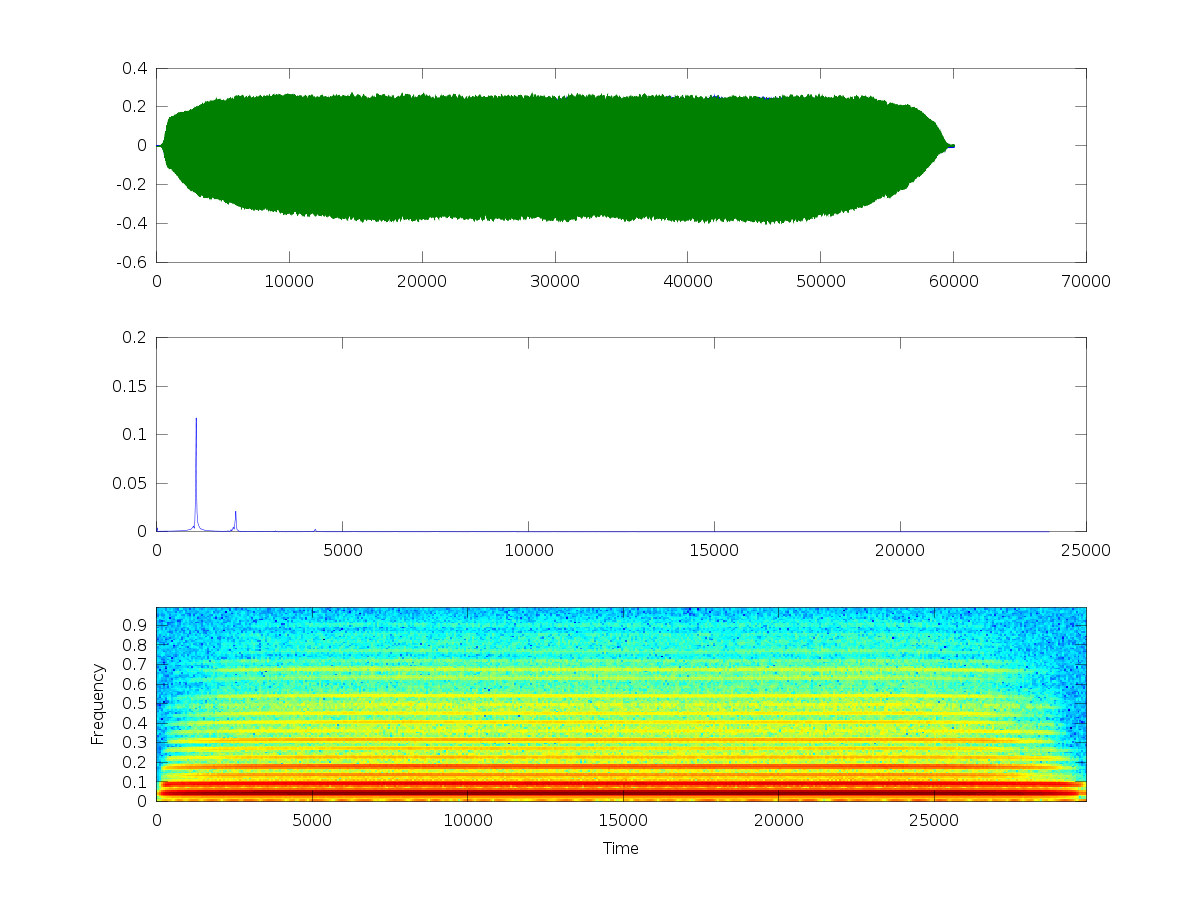
\includegraphics[scale=0.5]{proba1_flet.png}
\caption{Flet}
\label{fig:flet}
\end{figure}
\begin{figure}
\hspace{-10em}
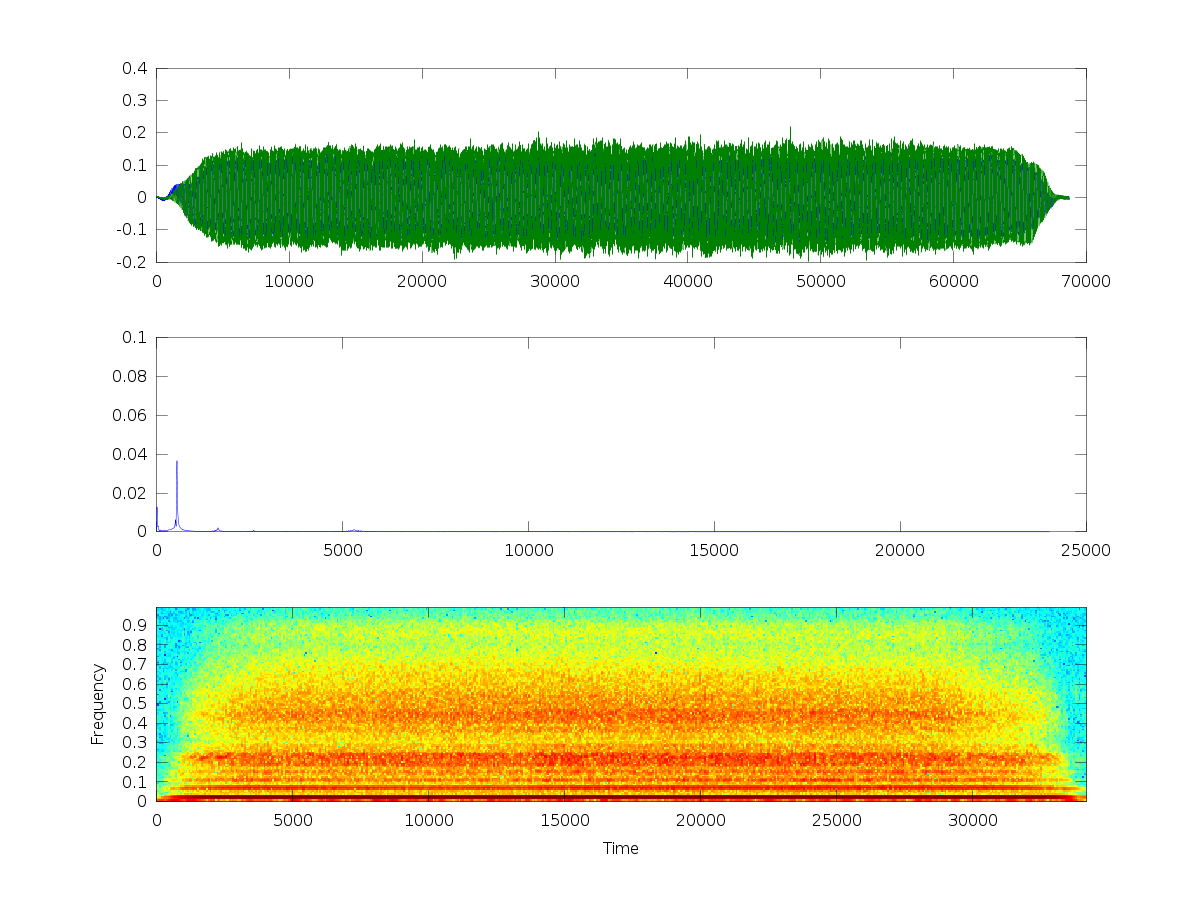
\includegraphics[scale=0.5]{proba1_fletnia.png}
\caption{Fletnia}
\label{fig:fletnia}
\end{figure}
\begin{figure}
\hspace{-10em}
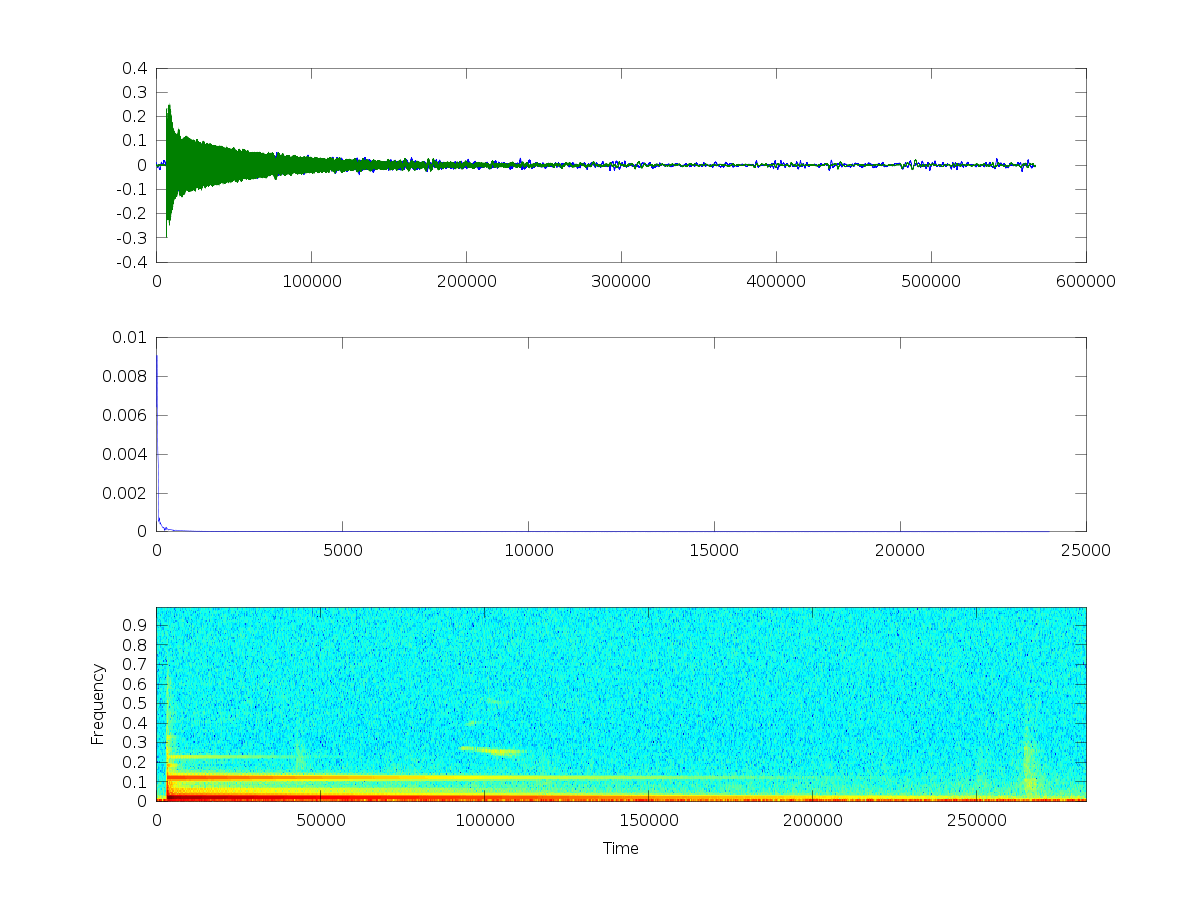
\includegraphics[scale=0.5]{proba1_kamerton.png}
\caption{Kamerton}
\label{fig:kamerton}
\end{figure}
\newpage
\item Naszym zadaniem jest wygenerowanie pogłosu oraz sygnału oryginalnego z~wyznaczonym pogłosem.\\
Powyższe zadanie realizuje poniższy program:
\lstinputlisting[language=Octave,basicstyle=\footnotesize,caption="Zadanie 2"]{zad2.m}
\end{enumerate}
\end{document}
